\documentclass[letterpaper, reqno,11pt]{article}
\usepackage[margin=1.0in]{geometry}
\usepackage{color,latexsym,amsmath,amssymb,graphicx,float,listings,tikz}
\usepackage{hyperref}

\hypersetup{
colorlinks=true,
linkcolor=magenta,
filecolor=magenta,
urlcolor=cyan,
}

\graphicspath{ {images/} }

\begin{document}
\pagenumbering{arabic}
\title{Math 443 Homework 10}
\date{12/04/23}
\author{Xander Naumenko}
\maketitle

{\medskip\noindent\bf Question 1.} The chromatic coloring is 4. As seen in figure \ref{fig:1}, the graph is planar, so it has $\chi\left( G \right)\leq 4$. Since $K_3$ is an induced subgraph we also have that $\chi(G)\geq 3$. To see why it can't be 3, consider figure \ref{fig:1}. By contradiction assume that it was 3-colorable. Without loss of generality color vertices $a,b,c$ with red, green and blue respectively. Then $d$ must be green, $e$ must be blue and $f$ is green, but this is a contradiction since $b$ is also green. Thus it couldn't have been 3-colorable and the only possibility is that $\chi(G)=4$.

\begin{figure}[htpb]
    \centering
    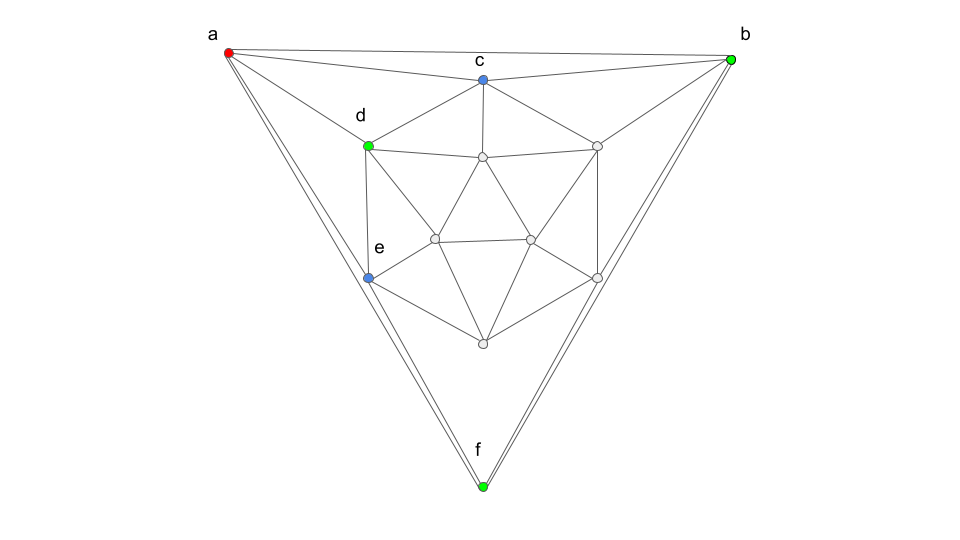
\includegraphics[width=0.8\textwidth]{1}
    \caption{Contradiction proof sketch for question 1.}
    \label{fig:1}
\end{figure}

{\medskip\noindent\bf Question 2.} The map is 3 colorable, see figure \ref{fig:2}. Since there is a $K_3$ is a subgraph it must also be at least 3, so $\chi(\text{Canada})=3$.

\begin{figure}[htpb]
    \centering
    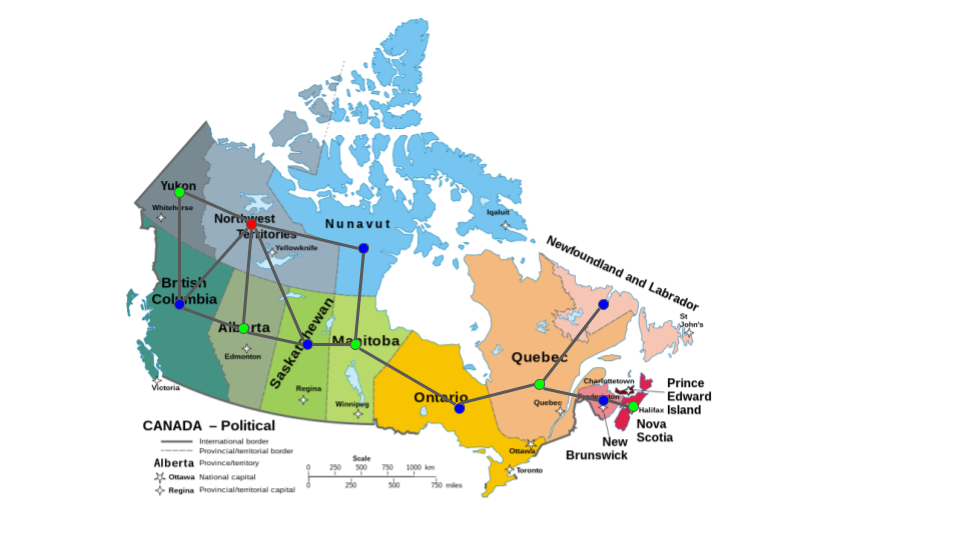
\includegraphics[width=0.8\textwidth]{2}
    \caption{Map of Canada, vertex colors are graph coloring, not region coloring.}
    \label{fig:2}
\end{figure}

{\medskip\noindent\bf Question 3a.} $\chi(G)=3$. $G$ contains $K_3$ as a subgraph, so $\chi\geq 3$. As seen in figure \ref{fig:3a} we also have that $\chi(G)\leq 3$ since we found an example of a 3 coloring. Thus $\chi(G)=3$.

\begin{figure}[htpb]
    \centering
    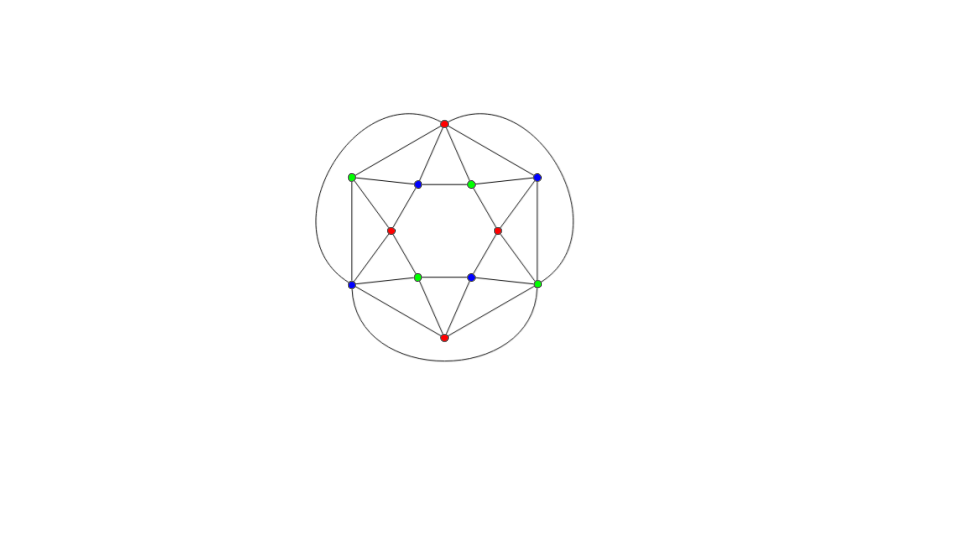
\includegraphics[width=0.8\textwidth]{3a}
    \caption{Coloring for question 3a.}
    \label{fig:3a}
\end{figure}

{\medskip\noindent\bf Question 3b.} The minimum number is 2. Clearly it's at least 2, since there is more than two regions. We can also see that there is an example of a 2-region-coloring in figure \ref{fig:3b}. Thus the minimum number is 2.

\begin{figure}[htpb]
    \centering
    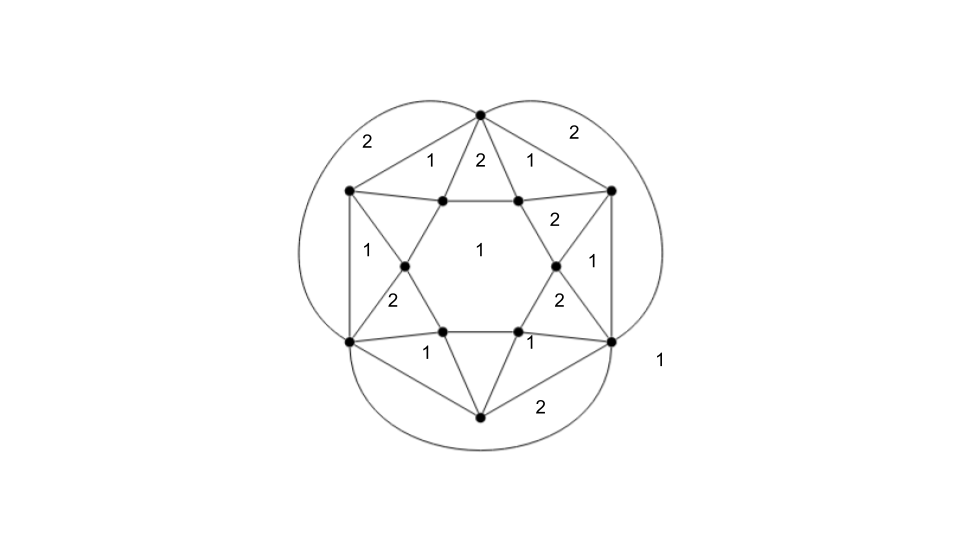
\includegraphics[width=0.8\textwidth]{3b}
    \caption{Coloring for regions of 3b.}
    \label{fig:3b}
\end{figure}

{\medskip\noindent\bf Question 3c.} The answer is $\chi'(G)=6$. Although justification isn't required, one such coloring is in figure \ref{fig:3c}.

\begin{figure}[htpb]
    \centering
    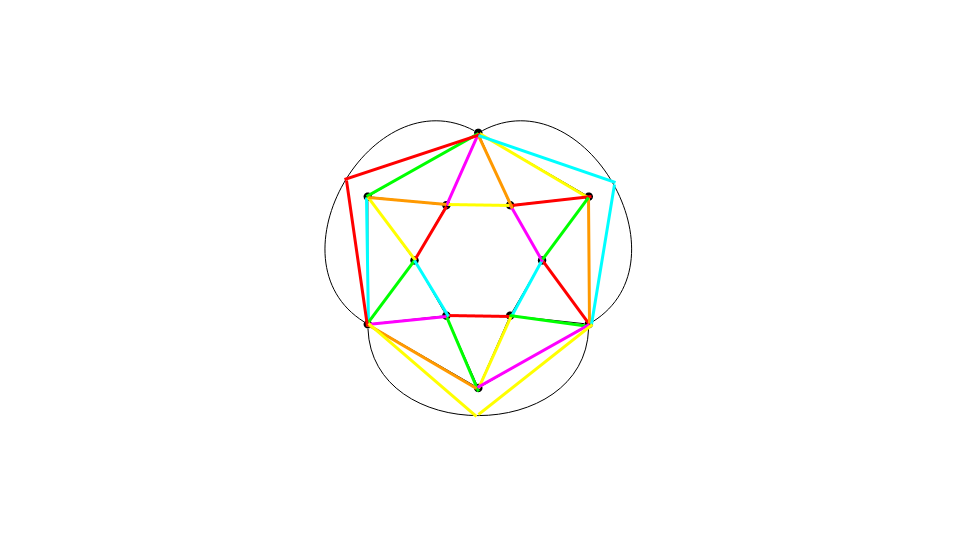
\includegraphics[width=0.8\textwidth]{3c}
    \caption{Coloring for question 3c.}
    \label{fig:3c}
\end{figure}

\end{document}
